\documentclass{article}

% if you need to pass options to natbib, use, e.g.:
% \PassOptionsToPackage{numbers, compress}{natbib}
% before loading nips_2016
%
% to avoid loading the natbib package, add option nonatbib:
% \usepackage[nonatbib]{nips_2016}

\usepackage[final]{nips_2016}

% to compile a camera-ready version, add the [final] option, e.g.:
% \usepackage[final]{nips_2016}

\usepackage[utf8]{inputenc} % allow utf-8 input
\usepackage[T1]{fontenc}    % use 8-bit T1 fonts
\usepackage{hyperref}       % hyperlinks
\usepackage{url}            % simple URL typesetting
\usepackage{booktabs}       % professional-quality tables
\usepackage{amsfonts}       % blackboard math symbols
\usepackage{nicefrac}       % compact symbols for 1/2, etc.
\usepackage{microtype}      % microtypography
\usepackage{physics}		 % Physics package for derivatives
\usepackage{graphicx,float,caption,subcaption,tikz}
\usepackage{listings}
\usepackage{color} %red, green, blue, yellow, cyan, magenta, black, white
\usepackage{animate}
\usepackage{multirow}
\usepackage{pgffor}
\usepackage{tabularx}

\usepackage{amsmath}
\usepackage{latexsym}
\usepackage{amssymb}
\usepackage{mathtools}
\usepackage{bm}
\usepackage{array}
\captionsetup[table]{skip=10pt}

\DeclareMathOperator*{\argmax}{\arg\max}
\DeclareMathOperator*{\argmin}{\arg\min}
\DeclareMathOperator*{\E}{\mathbb{E}}

\bibliographystyle{abbrvnat}
\graphicspath{ {results/} }

\newcounter{codenum}
\newcounter{imgnum}
\makeatletter
\newtoks\@tabtoks
\newcommand\addtabtoks[1]{\global\@tabtoks\expandafter{\the\@tabtoks#1}}
\newcommand\eaddtabtoks[1]{\edef\mytmp{#1}\expandafter\addtabtoks\expandafter{\mytmp}}
\newcommand*\resettabtoks{\global\@tabtoks{}}
\newcommand*\printtabtoks{\the\@tabtoks}
\makeatother

\title{Computer Vision Report: Text to Image Synthesis}

% The \author macro works with any number of authors. There are two
% commands used to separate the names and addresses of multiple
% authors: \And and \AND.
%
% Using \And between authors leaves it to LaTeX to determine where to
% break the lines. Using \AND forces a line break at that point. So,
% if LaTeX puts 3 of 4 authors names on the first line, and the last
% on the second line, try using \AND instead of \And before the third
% author name.

\author{
  Ankit Vani \\
  \texttt{ankit.vani@nyu.edu} \\
  \And
  Srivas Venkatesh \\
  \texttt{srivas.venkatesh@nyu.edu} \\
}

\begin{document}

\maketitle

\begin{abstract}
Generative adversarial networks have been shown to generate very realistic images by learning through a min-max game. Furthermore, these models are known to model image spaces more easily when conditioned on class labels. In this work, we consider conditioning on fine-grained textual descriptions, thus also enabling us to produce realistic images that correspond to the input text description. Additionally, we consider the task of learning disentangled representations for images through special latent codes, such that we can move them as knobs to alter the generated image. These latent codes take on very interpretable roles and are learnt in a completely unsupervised manner, using ideas from InfoGAN. We show that the learnt latent codes that encode much more variance and semantic interpretability as compared to standard GANs by experimenting on two datasets.
\end{abstract}


\section{Introduction}

Building models of our complex real world is a fascinating and a very difficult problem. In this project, we tackle the problem of modeling concepts from textual data, and mapping them to the image space. We use generative adversarial networks (GANs) (\cite{gan}) to generate realistic images from raw textual descriptions. However, to go one step further, we also wish to learn disentangled representations of images that can be used to adjust the generated images in an interpretable way. Ideally, we would want a small number of controls to do so, rather than hundreds of knobs with no idea how those variables interact with each other.

To achieve this, we consider the information theoretic extension of GAN, known as InfoGAN (\cite{infogan}), to maximize the mutual information between certain latent codes and the image generated from them. We extend the previous text to image work (\cite{text2image}) using InfoGAN, and extend InfoGAN by conditioning on textual representations. We find that these latent codes can learn to pick up global semantics from the data distribution, so that once they are learnt, they can be labeled by the interpretable effect they have on the image to enable manual fine-tuning after generating an image from its caption.


\section{Background}

\subsection{Generative Adversarial Network (GAN)}

Generative Adversarial Networks (GANs) (\cite{gan}) have been tremendously successful in learning to generate realistic images by playing a min-max game. A discriminator $D$ is trained to classify input images as coming from the data distribution (`real') or coming from the generator (`fake'). A generator $G$ is trained to fool the discriminator by producing images that are indistinguishable from real images for the discriminator. The generator takes as input a noise vector $z$, coming from a prior distribution, and maps it to a point in the pixel space, which represents an image. The prior noise distribution usually has zero mean and is a Gaussian or a uniform distribution.

The GAN objective can thus be formulated as
\begin{align}
\min_G \max_D\, V(D,G) = \E_{x \sim p_{\text{data}}(x)}\left[\log D(x)\right] + \E_{z\sim p_z(z)}\left[\log(1-D(G(z)))\right] \label{eq:gan}
\end{align}

The signal for the generator to update its generative model comes from the discriminator itself, by using gradients of the discriminator loss with respect to the generated image. In practice, gradients from the discriminator are reversed and backpropagated to the generator, thereby asking the generator to maximize the discriminator's loss.


\subsection{Deep Convolutional GAN (DCGAN)}

To get better quality generations from the generators of GANs, \cite{dcgan} presented an architecture called deep convolutional GAN (DCGAN) where the generator and the discriminator are convolutional networks that mirror each other in structure.

They also replace the pooling layers with strided convolutions in the discriminator and fractional-strided convolutions in the generator. Additionally, they use the LeakyReLU activation in the discriminator for all layers instead of ReLU. These two additions ensure that there are no sparse gradients in the discriminator, which helps with the stability of the min-max objective training. To alleviate internal covariate shift and help make training more stable, they use batch normalization (\cite{batchnorm}) in both the generator and the discriminator. There are no fully connected hidden layers, enabling deeper models.

The text to image architecture we use is based on the DCGAN architecture.



\subsection{Information Maximizing GAN (InfoGAN)}

Information maximizing GAN (InfoGAN) (\cite{infogan}) is an extension to GAN that learns disentangled representations in an unsupervised manner. Unlike the standard GAN, where an image is generated from a noise vector $z$, an image in this case is generated from a noise vector $z$ and latent codes $c$. Like $z$, we define a prior distribution over $c$ with zero mean, which is usually taken to be a Gaussian or a uniform distribution. $c$ can also contain discrete latent codes, which can have a discrete uniform prior.

To learn disentangled representations, the model maximizes the mutual information between $c$ and the generated image $G(z,c)$, where the mutual information is given by
\begin{align}
\mathcal{I}(c;G(z,c)) = \mathcal{H}(G(z,c)) - \mathcal{H}(G(z,c) \mid c) = \mathcal{H}(c) - \mathcal{H}(c\mid G(z,c)) \label{eq:mi}
\end{align}

The authors derive a variational lower bound to Equation (\ref{eq:mi}):
\begin{align}
\mathcal{I}(c;G(z,c)) &\geq \E_{x\sim G(z,c)}\left[\E_{c'\sim p(c\mid x)}\left[\log Q(c'\mid x)\right]\right] + \mathcal{H}(c) \label{eq:milb}
\end{align}
where $Q$ is a variational approximation for $p(c\mid x)$. They show that under suitable regularity conditions, Equation (\ref{eq:milb}) can be simplified to
\begin{align}
\mathcal{I}(c;G(z,c)) &\geq \E_{c\sim p(c), x\sim G(z,c)}\left[\log Q(c\mid x)\right] + \mathcal{H}(c) = L_I(G,Q) \label{eq:miloss}
\end{align}

Thus, by maximizing $L_I(G,Q)$, we would maximize the mutual information between $c$ and $G(z,c)$. $L_I$ can be added to the GAN's objective and maximized jointly with respect to $G$ and $Q$ as
\begin{align}
\min_{G,Q} \max_D\, V_{\text{InfoGAN}}(D,G,Q) = V(D,G) - \lambda L_I(G,Q)
\end{align}
where $V(D,G)$ is defined in Equation (\ref{eq:gan}). $\lambda$ is a hyperparameter, that is tuned to weigh the mutual information criterion in the learning objective. The authors suggest setting this value such that $\lambda L_I$ is on the same scale as the GAN objective $V$.

In practice, $Q$ shares all of its layers and parameters with $D$ upto $D$'s penultimate layer, following with an additional layer that outputs the sufficient statistics of the distribution $Q(c\mid x)$. For a Gaussian, these are the mean and diagonal covariance values. For discrete latent codes, these are the softmax logits. $Q$ converges very quickly during training, and thus it essentially comes for free with GAN, without the need for additional training time or model capacity beyond a single layer.


\subsection{Deep symmetric structured joint embedding}

Given an image $v\in\mathcal{V}$ and its corresponding fine-grained textual description $t\in\mathcal{T}$, \cite{visualdesc} suggest learning the encodings $\theta(v)$ for images and $\varphi(t)$ for text, such that a joint embedding $F(v,t)=\theta(v)^\top \varphi(t)$ can be defined. They define the classifiers
\begin{align}
f_v(v) &= \argmax_{y\in\mathcal{Y}} \E_{t\in\mathcal{T}(y)}\left[F(v,t)\right],\\
f_t(t) &= \argmax_{y\in\mathcal{Y}} \E_{v\in\mathcal{V}(y)}\left[F(v,t)\right]
\end{align}
to classify data points $(v,t)$ into labels $y\in\mathcal{Y}$. By jointly training the text and image encoders to minimize the classification loss, they are able to learn visually descriptive embeddings $\varphi(t)$ for text and embeddings $\theta(v)$ for images, such that they have a higher compatibility score $F$ when their class is the same.

They explore various text encoder models, such as a convolutional network, a convolutional recurrent network and a recurrent network. For our work on text to image synthesis, we use pretrained text encoders provided by the authors, that use a character-level convolutional recurrent network.


\section{Text to Image InfoGAN}

\subsection{Objective}

Text to Image GAN (\cite{text2image}) is a conditional GAN, where the discriminator $D$ and the generator $G$ are conditioned on a text encoding $\varphi(t)$ for an image caption $t$. Thus, given a text caption, the generator is tasked with producing a realistic image described by the input caption. When training the generator, the authors also propose creating auxiliary text embeddings by interpolating between embeddings of text descriptions in the data, essentially providing infinite samples from the text embedding space to condition on.

Based on Equation (\ref{eq:gan}), we can formulate the text to image GAN objective as
\begin{align}
\min_G \max_D\, \mathcal{V}(D,G, \varphi) =& \E_{(x,t) \sim p_{\text{data}}(x,t)}\left[\log D(x, \varphi(t))\right]\, + \nonumber\\
&\E_{z\sim p_z(z), t\sim p_{\text{intdata}}(t)}\left[\log(1-D(G(z, \varphi(t)), \varphi(t)))\right] \label{eq:t2i}
\end{align}
where $t \sim p_{\text{intdata}}(t)$ is short for sampling through the process $t_1 \sim p_{\text{data}}(t), t_2 \sim p_{\text{data}}(t), \beta \sim [0,1], t = \beta t_1 + (1-\beta) t_2$.

We extend the text to image GAN by adding the ability to manipulate the output images, adjusting it manually to possibly better suit the textual description. We learn disentangled latent codes $c$, enabling each latent code to take on interpretable and semantically meaningful roles. We do this by extending InfoGAN to the text to image synthesis setting, where we want to maximize the mutual information between the latent codes $c$ and the conditionally generated image $G(z,c,\varphi(t))$:
\begin{align}
\mathcal{I}(c;G(z,c,\varphi(t))) &\geq \E_{t\sim p_{\text{intdata}}(t), x\sim G(z,c,\varphi(t))}\left[\E_{c'\sim p(c\mid x,t)}\left[\log Q(c'\mid x,t)\right]\right] + \mathcal{H}(c)
\end{align}

As described for InfoGAN, under suitable regularity conditions, we can obtain a variational lower bound for $\mathcal{I}(c;G(z,c,\varphi(t)))$:
\begin{align}
\mathcal{I}(c;G(z,c, \varphi(t))) &\geq \E_{c\sim p(c), t\sim p_{\text{intdata}}(t), x\sim G(z,c, \varphi(t))}\left[\log Q(c\mid x,t)\right] + \mathcal{H}(c) = \mathcal{L}_I(G,Q,\varphi) \label{eq:t2imiloss}
\end{align}

We experiment with two possible models, one where the variational approximation $Q$ takes into consideration the textual description when looking at the generated image, and one where it doesn't. In the case where $Q$ does not consider the textual description, we assume in Equation (\ref{eq:t2imiloss}) that the output of $Q$ is conditionally independent of $t$ given $x$, in which case $Q(c\mid x,t)$ simplifies to $Q(c\mid x)$. This is equivalent to removing an edge between $t$ and $c$ sampled from $Q$ in the graphical model.

Our text to image InfoGAN objective is given by
\begin{align}
\min_{G,Q} \max_D\, \mathcal{V}_{\text{t2i2GAN}}(D,G,Q,\varphi) = \mathcal{V}(D,G,\varphi) - \lambda \mathcal{L}_I(G,Q,\varphi)
\end{align}
where $\mathcal{V}(D,G,\varphi)$ is defined in Equation (\ref{eq:t2i}), and $\mathcal{L}_I(G,Q,\varphi)$ in Equation (\ref{eq:t2imiloss}).


\subsection{Model architecture}

\begin{figure}
    \centering
    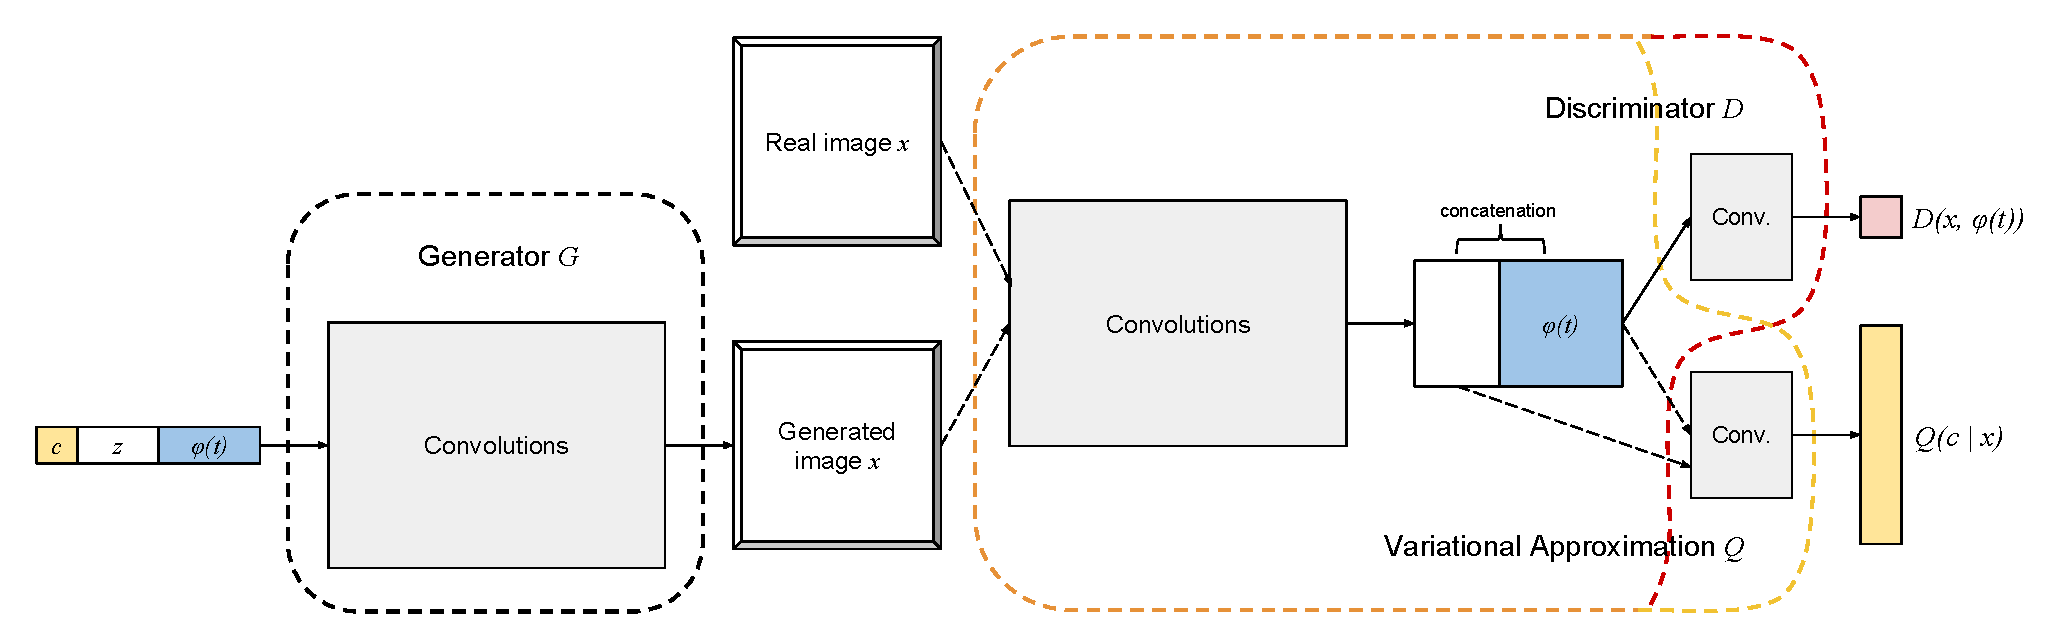
\includegraphics[width=\textwidth]{arch}
    \caption{High-level architecture for Text to Image InfoGAN model. The grey convolution blocks abstract the DCGAN architecture. Dashed arrows represent alternate flows.}
    \label{fig:arch}
\end{figure}

Our model architecture is very similar to \cite{text2image}, which itself is based on the DCGAN architecture. The generator and the discriminator are both conditioned on the text embedding $\varphi(t)$, which comes from the data distribution in case the discriminator is looking at a real image, or from interpolations of true text embeddings in case of generations. Our model architecture is illustrated in Figure \ref{fig:arch}.

The generator takes as input a vector formed by the concatenation of latent codes $c$, noise $z$, and the text embedding. We choose the prior for $z$ to be a Gaussian with zero mean and identity covariance. We sample $c$ from a multivariate uniform distribution between $-1$ and $1$, but consider the prior $p(c)$ to be a Gaussian with zero mean and identity covariance for the mutual information lower bound defined in Equation (\ref{eq:t2imiloss}). The text embedding $\varphi(t)$ is passed through a fully-connected network and reduced to a size of 128 dimensions, followed by a LeakyReLU, before concatenation to the input vector.

Another transformation on the text embedding $\varphi(t)$ followed by rectification is done for the discriminator. When the spatial dimension of the DCGAN discriminator is $4\times 4$, we replicate this reduced embedding spatially and concatenate it to the $4\times 4$ discriminator output. A $1\times 1$ convolution followed by rectification and another $4\times 4$ convolution is performed obtain the final discriminator value.

If we want to consider $Q(c\mid x,t)$ (that is, consider the textual description in $Q$ in addition to the generated image), then the depth concatenated $4\times 4$ output is passed through a different $1\times 1$ convolution followed by rectification. The output is then flattened and a fully connected layer maps it to a vector representing the mean and diagonal covariance for the latent codes in $Q(c\mid x,t)$. If we instead want to only consider $Q(c\mid x)$, then we use the $4\times 4$ discriminator output before depth concatenation for the convolutional layer of $Q$.




\section{Experimental Results}
\subsection{Datasets}
For our experiments, we used 2 datasets: 
\begin{itemize}
    \item The Caltech University Birds Dataset (\cite{cub})

         It is an image
        dataset with 6033 photos of 200 bird species. It also contains details
        such as species label, bounding boxes, segmentation and positional
        attributes which we don't use for our purposes.
    \item The Oxford Flowers Dataset (\cite{flowers})
    
       It is an image dataset of
        102 flower categories with between 40 to 358 images per category. It
        also contains class labels, segmentation masks which we don't make use
        of for our problem.
\end{itemize}
We do however need text captions for these datasets which we obtain from the data
curated by \cite{visualdesc}.

\subsection{Conditioning image generation with captions}
We aim to compare the latent codes used to generate the images by \cite{text2image} with our model. In the original model, it has been shown that the text
encodings capture the image content whereas the latent noise vector captures the
style of the image such as orientation, background, etc. However to illustrate
this, \cite{text2image} invert the generator to obtain the
noise code $z$ for similar images (based on bird orientation, background color
etc) and shows that they have similar noise vectors and that the style can be
transferred to other images by simply changing the text encodings. However the
style isn't completely disentangled as it is present in very high dimensional
space. This can be seen in the Table \ref{table:cub} where variations of the first 5
dimensions of the latent codes don't really offer any drastic style change.

\begin{table}[H]
\begin{tabularx}{\textwidth}{|c|X|X|X|X|X|}
\hline
Latent Code & -2 & -1 & 0 & 1 & 2\\
\hline
1 & 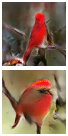
\includegraphics[keepaspectratio,width=0.7\hsize]{base_full_btch2/img_1_1_1} & 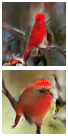
\includegraphics[keepaspectratio,width=0.7\hsize]{base_full_btch2/img_1_1_2} & 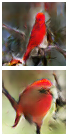
\includegraphics[keepaspectratio,width=0.7\hsize]{base_full_btch2/img_1_1_3} & 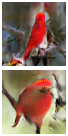
\includegraphics[keepaspectratio,width=0.7\hsize]{base_full_btch2/img_1_1_4} & 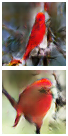
\includegraphics[keepaspectratio,width=0.7\hsize]{base_full_btch2/img_1_1_5} \\\hline
2 & 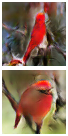
\includegraphics[keepaspectratio,width=0.7\hsize]{base_full_btch2/img_1_2_1} & 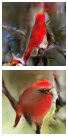
\includegraphics[keepaspectratio,width=0.7\hsize]{base_full_btch2/img_1_2_2} & 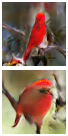
\includegraphics[keepaspectratio,width=0.7\hsize]{base_full_btch2/img_1_2_3} & 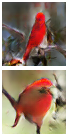
\includegraphics[keepaspectratio,width=0.7\hsize]{base_full_btch2/img_1_2_4} & 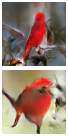
\includegraphics[keepaspectratio,width=0.7\hsize]{base_full_btch2/img_1_2_5} \\\hline
3 & 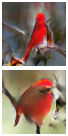
\includegraphics[keepaspectratio,width=0.7\hsize]{base_full_btch2/img_1_3_1} & 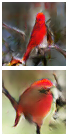
\includegraphics[keepaspectratio,width=0.7\hsize]{base_full_btch2/img_1_3_2} & 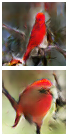
\includegraphics[keepaspectratio,width=0.7\hsize]{base_full_btch2/img_1_3_3} & 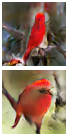
\includegraphics[keepaspectratio,width=0.7\hsize]{base_full_btch2/img_1_3_4} & 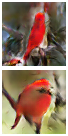
\includegraphics[keepaspectratio,width=0.7\hsize]{base_full_btch2/img_1_3_5} \\\hline
4 & 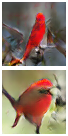
\includegraphics[keepaspectratio,width=0.7\hsize]{base_full_btch2/img_1_4_1} & 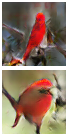
\includegraphics[keepaspectratio,width=0.7\hsize]{base_full_btch2/img_1_4_2} & 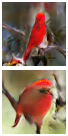
\includegraphics[keepaspectratio,width=0.7\hsize]{base_full_btch2/img_1_4_3} & 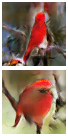
\includegraphics[keepaspectratio,width=0.7\hsize]{base_full_btch2/img_1_4_4} & 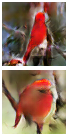
\includegraphics[keepaspectratio,width=0.7\hsize]{base_full_btch2/img_1_4_5} \\\hline
5 & 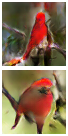
\includegraphics[keepaspectratio,width=0.7\hsize]{base_full_btch2/img_1_5_1} & 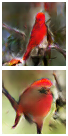
\includegraphics[keepaspectratio,width=0.7\hsize]{base_full_btch2/img_1_5_2} & 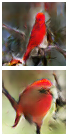
\includegraphics[keepaspectratio,width=0.7\hsize]{base_full_btch2/img_1_5_3} & 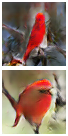
\includegraphics[keepaspectratio,width=0.7\hsize]{base_full_btch2/img_1_5_4} & 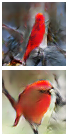
\includegraphics[keepaspectratio,width=0.7\hsize]{base_full_btch2/img_1_5_5} \\\hline
\end{tabularx}
\caption{Table of generated images with change of the first 5 latent code
dimensions from -2 to 2 for the original model.}
\label{table:cub}
\end{table}
In Table \ref{table:cub} we use the query text ``this vibrant red bird has a pointed
black beak''. We shall continue to use the same query to make meaningful
comparisons.

\subsection{Effect of the mutual information criterion}
By incorporating the mutual information maximization objective, our
model succeeds in disentangling the style variable onto distinct dimensions of the
noise vector. In fact, on the birds dataset, it manages to disentangle all the
style/content factors mentioned in \cite{text2image} such as orientation, shape
and background. The network learns to disentangle these factors onto the latent
dimensions we try to maximize the mutual information with. Generations from this
model are shown in Table \ref{table:cub_mi}.
\begin{table}
\begin{tabularx}{\textwidth}{|c|X|X|X|X|X|}
\hline
Latent Code & -2 & -1 & 0 & 1 & 2\\
\hline
1 & \shortstack{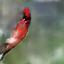
\includegraphics[keepaspectratio,width=0.7\hsize]{1a/img_c1_i1}\\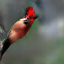
\includegraphics[keepaspectratio,width=0.7\hsize]{1b/img_c1_i1}} & \shortstack{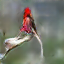
\includegraphics[keepaspectratio,width=0.7\hsize]{1a/img_c1_i2}\\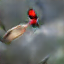
\includegraphics[keepaspectratio,width=0.7\hsize]{1b/img_c1_i2}} & \shortstack{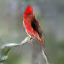
\includegraphics[keepaspectratio,width=0.7\hsize]{1a/img_c1_i3}\\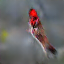
\includegraphics[keepaspectratio,width=0.7\hsize]{1b/img_c1_i3}} & \shortstack{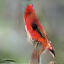
\includegraphics[keepaspectratio,width=0.7\hsize]{1a/img_c1_i4}\\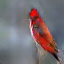
\includegraphics[keepaspectratio,width=0.7\hsize]{1b/img_c1_i4}} & \shortstack{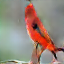
\includegraphics[keepaspectratio,width=0.7\hsize]{1a/img_c1_i5}\\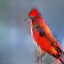
\includegraphics[keepaspectratio,width=0.7\hsize]{1b/img_c1_i5}} \\\hline
2 & \shortstack{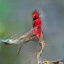
\includegraphics[keepaspectratio,width=0.7\hsize]{1a/img_c2_i1}\\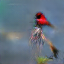
\includegraphics[keepaspectratio,width=0.7\hsize]{1b/img_c2_i1}} & \shortstack{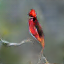
\includegraphics[keepaspectratio,width=0.7\hsize]{1a/img_c2_i2}\\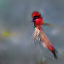
\includegraphics[keepaspectratio,width=0.7\hsize]{1b/img_c2_i2}} & \shortstack{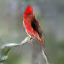
\includegraphics[keepaspectratio,width=0.7\hsize]{1a/img_c2_i3}\\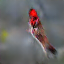
\includegraphics[keepaspectratio,width=0.7\hsize]{1b/img_c2_i3}} & \shortstack{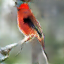
\includegraphics[keepaspectratio,width=0.7\hsize]{1a/img_c2_i4}\\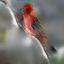
\includegraphics[keepaspectratio,width=0.7\hsize]{1b/img_c2_i4}} & \shortstack{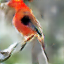
\includegraphics[keepaspectratio,width=0.7\hsize]{1a/img_c2_i5}\\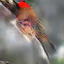
\includegraphics[keepaspectratio,width=0.7\hsize]{1b/img_c2_i5}} \\\hline
3 & \shortstack{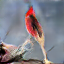
\includegraphics[keepaspectratio,width=0.7\hsize]{1a/img_c3_i1}\\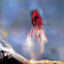
\includegraphics[keepaspectratio,width=0.7\hsize]{1b/img_c3_i1}} & \shortstack{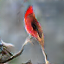
\includegraphics[keepaspectratio,width=0.7\hsize]{1a/img_c3_i2}\\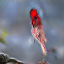
\includegraphics[keepaspectratio,width=0.7\hsize]{1b/img_c3_i2}} & \shortstack{\includegraphics[keepaspectratio,width=0.7\hsize]{1a/img_c3_i3}\\\includegraphics[keepaspectratio,width=0.7\hsize]{1b/img_c3_i3}} & \shortstack{\includegraphics[keepaspectratio,width=0.7\hsize]{1a/img_c3_i4}\\\includegraphics[keepaspectratio,width=0.7\hsize]{1b/img_c3_i4}} & \shortstack{\includegraphics[keepaspectratio,width=0.7\hsize]{1a/img_c3_i5}\\\includegraphics[keepaspectratio,width=0.7\hsize]{1b/img_c3_i5}} \\\hline
\end{tabularx}
\caption{Table of generated images with change of the designated 3 continuous
latent code dimensions from -2 to 2 for our model.}
\label{table:cub_mi}
\end{table}
As we can see in Table \ref{table:cub_mi}, the first dimension has learnt to
disentangle the direction the bird is facing, the second dimension has learnt to disentangle the bird's size, and the third dimension has learnt to disentangle the background.

Our model accomplishes the same effect in the flowers dataset as well. The
latent code disentangling of the flowers dataset is shown in Table \ref{table:flowers_mi}.
\begin{table}
\begin{tabularx}{\textwidth}{|c|X|X|X|X|X|}
\hline
Latent Code & -2 & -1 & 0 & 1 & 2\\
\hline
1 & \includegraphics[keepaspectratio,width=0.7\hsize]{flowers_3c_5d_l01_notxt_btch2/img_2_1_1} & \includegraphics[keepaspectratio,width=0.7\hsize]{flowers_3c_5d_l01_notxt_btch2/img_2_1_2} & \includegraphics[keepaspectratio,width=0.7\hsize]{flowers_3c_5d_l01_notxt_btch2/img_2_1_3} & \includegraphics[keepaspectratio,width=0.7\hsize]{flowers_3c_5d_l01_notxt_btch2/img_2_1_4} & \includegraphics[keepaspectratio,width=0.7\hsize]{flowers_3c_5d_l01_notxt_btch2/img_2_1_5} \\\hline
2 & \includegraphics[keepaspectratio,width=0.7\hsize]{flowers_3c_5d_l01_notxt_btch2/img_2_2_1} & \includegraphics[keepaspectratio,width=0.7\hsize]{flowers_3c_5d_l01_notxt_btch2/img_2_2_2} & \includegraphics[keepaspectratio,width=0.7\hsize]{flowers_3c_5d_l01_notxt_btch2/img_2_2_3} & \includegraphics[keepaspectratio,width=0.7\hsize]{flowers_3c_5d_l01_notxt_btch2/img_2_2_4} & \includegraphics[keepaspectratio,width=0.7\hsize]{flowers_3c_5d_l01_notxt_btch2/img_2_2_5} \\\hline
3 & \includegraphics[keepaspectratio,width=0.7\hsize]{flowers_3c_5d_l01_notxt_btch2/img_2_3_1} & \includegraphics[keepaspectratio,width=0.7\hsize]{flowers_3c_5d_l01_notxt_btch2/img_2_3_2} & \includegraphics[keepaspectratio,width=0.7\hsize]{flowers_3c_5d_l01_notxt_btch2/img_2_3_3} & \includegraphics[keepaspectratio,width=0.7\hsize]{flowers_3c_5d_l01_notxt_btch2/img_2_3_4} & \includegraphics[keepaspectratio,width=0.7\hsize]{flowers_3c_5d_l01_notxt_btch2/img_2_3_5} \\\hline
\end{tabularx}
\caption{Table of generated images for the flowers dataset with change of the
    designated 3 continuous latent code dimensions from -2 to 2 for our model.}
\label{table:flowers_mi}
\end{table}
In Table \ref{table:flowers_mi} we use the query text ``the center is yellow surrounded by
wavy dark purple petals''. We see that in the case of the flowers dataset, it has
learnt to disentangle elevation of the flower on the first dimension, rotation
of the flower with respect to the stem is captured by the second dimension and
the elongation along $-45$/$+45$ degree axis is captured by the the third dimension.

\subsection{Other Experiments}
For this task we have a couple of hyperparameters which had to be tuned to give
relevant results. Some of these are detailed below along with some values we
tried for them:
\begin{itemize}
    \item The Number of continuous latent codes to apply the mutual information
        criteria on
        
        Ideally this should be decided based on the structure of
        the data. For our case, we started of with 5 continuous latent codes to
        realize that only 3 of those were identifying distinct features such as
        orientation, background and size. The other 2 were learning a
        combination of these 3 on the birds dataset. Hence we decided to use 3
        continuous latent codes for the mutual information criterion. We decided
        to use the same number for the flowers dataset as well as there were
        only about so much variation in that dataset as well.
    \item Weight of the mutual information criteria $\lambda$
    
    We want the
        mutual information criteria to be scaled by a factor such that it falls
        in the scale of the generator and discriminator losses. This avoids the
        mutual information criteria from dominating the losses, which in turn
        would affect the stability of the adversarial network. For our problem, we noticed that the
        mutual information criteria was about 3-10 times larger than the
        generator/discriminator losses and hence we tested with $\lambda = 0.1$,
        $\lambda = 0.3$. Both these gave similar results as far as resultant
        generations are concerned.

    \item Conditioning $Q$ on the text embeddings

    We found that choosing to condition $Q$ on the text embeddings or not made little difference in the latent code semantics learnt. Even when explicitly providing the text embeddings to the subnetwork that estimates $Q(c\mid x,t)$, the latent codes learnt to capture the same meanings as the ones where $Q$ is conditioned only on the generated image.

\end{itemize}

\subsection{Convergence of the mutual information criterion}
As indicated in InfoGAN (\cite{infogan}) the mutual information criterion quickly maximizes to
a value of around 8-10 depending on the dataset and our choice of $\lambda$.
This indicates that the bound is tight and that our network maximizes the mutual
information quite efficiently. This is shown in the figure \ref{fig:miplot} for some of our
experiments.
\begin{figure}
\centering
\includegraphics[width=0.7\textwidth]{miplot}
\caption{Plot of the mutual information between latent codes and generated image vs. epochs.}
\label{fig:miplot}
\end{figure}
\subsection{More examples and generalizations}
We present more examples to indicate that the latent code interpretation
generalizes to all examples. This indicates that style transfer is very easy
given these latent codes. We also present examples where the text descriptions
are made realistic yet very different from any caption present in the dataset to
see how the model generalizes to unknown examples. These are shown in Fig
\ref{animation} - Fig \ref{animation_flower}

\textit{Note: In interest of space and for better visualization the examples are
presented as animations. Please open in Acrobat Reader to view the same.}
\begin{figure}
\animategraphics[loop,controls,autoplay,width=\textwidth]{6}{cub_3c_2d_l01_txt/img_5_1_}{1}{10}
\animategraphics[loop,controls,autoplay,width=\textwidth]{6}{cub_3c_2d_l01_txt/img_5_2_}{1}{10}
\animategraphics[loop,controls,autoplay,width=\textwidth]{6}{cub_3c_2d_l01_txt/img_5_3_}{1}{10}
\caption{The generations of birds for the text 'a white bird with a very long
neck and a small red beak.' with variation of each of the 3 latent codes in
order}
\label{animation}
\end{figure}
\begin{figure}
\animategraphics[loop,controls,autoplay,width=\textwidth]{6}{flowers_3c_5d_l01_notxt/img_4_1_}{1}{10}
\animategraphics[loop,controls,autoplay,width=\textwidth]{6}{flowers_3c_5d_l01_notxt/img_4_2_}{1}{10}
\animategraphics[loop,controls,autoplay,width=\textwidth]{6}{flowers_3c_5d_l01_notxt/img_4_3_}{1}{10}
\caption{The generations of flowers for the text 'a very large flower with white petals with a splash of yellow color that extend in the veins toward the tips of the petal' with
    variation of each of the 3 latent codes in
order}
\label{animation_flower}
\end{figure}
\section{Conclusion}

Our goal was to use a textual description to generate an image corresponding to it, and then adjust it to get reasonable generations. To minimize the number of knobs we need to move to make such adjustments, we considered using the InfoGAN idea to maximize the mutual information between latent codes and the generated image.

We experimented with the Caltech University Birds dataset and the Oxford Flowers dataset, and showed that we are able to learn disentangled and interpretable semantic roles for each latent code. We compare our interpolations to interpolations without the mutual information criterion, and observed that the latent codes encode much more variance suitable for interpretable exploration of the image space.



\section*{Source code}

We started our implementation from Scott Reed's original codebase for Text to Image Synthesis, from \url{https://github.com/reedscot/icml2016}.

Our final codebase can be found at \url{https://github.com/alemc2/text2img}. The \texttt{README.md} file in the code repository explains how to learn the model and generate images for queries.

\begin{figure}
    \centering
    \includegraphics[width=0.8\textwidth]{web}
    \caption{A screenshot of a web interface to move sliders to adjust generated images from the caption. The sliders change the values of the latent codes.}
    \label{fig:web}
\end{figure}

You can also choose to enable the argument \texttt{web} of \texttt{txt2img\_demo.lua} to start a web server where you can submit a query, generate images from that query and then adjust those images with sliders representing their learnt latent codes. A screenshot of this web interface we developed is shown in Figure \ref{fig:web}.


\small
\bibliography{references}

\end{document}
